\section{Ziel}
\label{sec:Ziel}
In diesem Versuch sollen gekoppelte Schwingkreise auf ihren Energieübergang untersucht werden. Dazu werden die Frequenzabhängigkeiten des Stroms und die Fundamentalschwingungen mithilfe der Lissajous-Figuren 
in Abhängigkeit der Kopplung betrachtet.
\section{Theorie}
\label{sec:Theorie}
Ein System heißt \dq gekoppeltes\dq\; System, wenn es aus zwei Untersystemen
besteht, welche im gegenseitigem Energieaustausch stehen. Ein einfaches Beispiel für ein gekoppeltes System sind zwei gekoppelte Pendel. Die beiden Einzelpendel entsprechen dabei den Untersystemen.
Sie sind durch eine Feder gekoppelt, wodurch sie im gegenseitigen Energieaustausch stehen. In diesem Versuch werden anstatt gekoppelter Pendel kapazitiv gekoppelte Schwingkreise betrachtet.
Bei solchen Systemen ist es häufig von Interesse das Verhalten unter äußerer Anregung zu untersuchen.
\subsection{Kapazitiv gekoppelte Schwingkreise}
\label{T_KgS}
Nun wird ein Schwingkreise wie in \autoref{fig:T_skgS} betrachtet. Die Kopplung findet über den Kondensator $C_\text{K}$ statt, wodurch sich die beiden Schwingkreise das elektrische Feld dieses Kondensators
teilen. Durch die Kirchhoffschen Regeln lassen sich zwei unabhängige Differentialgleichungen aufstellen. Die Lösungen dieser beschreiben den überlagerten Stromverlauf,
sowie den Verlauf der Differenz des Stroms.
Die Summe der beiden Ströme $I_1$ und $I_2$ wird durch 
\begin{equation}
    \label{eqn:T_Iplus}
    \left(I_1 + I_2\right)\left(t\right) = \left(I_{1_0} + I_{2_0}\right)\frac{\text{cos}\left(t\right)}{\sqrt{LC}}
\end{equation}
beschrieben. Die Lösung der Differenz lautet
\begin{equation}
    \label{eqn:T_Iminus}
    \left(I_1 - I_2\right)\left(t\right) = \left(I_{1_0} - I_{2_0}\right)\text{cos}\left(\frac{t}{\sqrt{L\left(\frac{1}{C}+\frac{2}{C_k}\right)^{-1}}}\right).
\end{equation}
Aus \autoref{eqn:T_Iplus} und \autoref{eqn:T_Iminus} lassen sich die Schwingungsfrequenzen $\nu^+$ und $\nu^-$ aufstellen
\begin{equation}
    \label{eqn:T_nup}
    \nu^+ = \frac{1}{2\pi\sqrt{LC}}
\end{equation}
\begin{equation}
    \label{eqn:T_num}
    \nu^- =  \frac{1}{2\pi\sqrt{L\left(\frac{1}{C}+\frac{2}{C_k}\right)^{-1}}}.
\end{equation}
Des Weiteren lassen sich aus \autoref{eqn:T_Iplus} und \autoref{eqn:T_Iminus} die Stomverläufe $I_1(t)$ und $I_2(t)$ aufstellen. Durch Addition und Subtraktion der beiden genannten Gleichungen 
folgt 
\begin{equation}
    \label{T_I}
    I_{1,2}(t) = \frac{1}{2}\left(I_{1_0} + I_{2_0}\right)\text{cos}\left(2\pi\nu^+ t\right) - \frac{1}{2}\left(I_{1_0} - I_{2_0}\right)\text{cos}\left(2\pi\nu^- t\right).
\end{equation}
Betrachtet man nun den Fall der gleichsinnigen Schwingung $\left(I_{1_0} = I_{2_0}\right)$, fällt der Differenzteil der \autoref{T_I} weg und die Oszillatoren schwingen gleichphasig mit der Frequenz 
$\nu^+$.
Für den gegensinnigen Schwingfall $\left(I_{1_0} = -I_{2_0}\right)$ ergibt sich, dass die Oszillatoren gegenphasig mit der Frequenz $\nu^-$ schwingen.
Beim Schwebungsfall gilt zur Zeit $t = 0$ $I_{1_0}\neq 0$ und $I_{2_0} = 0$. Daraus ergibt sich für \autoref{T_I} 
\begin{equation*}
    I_1(t) = \frac{1}{2} I_{1_0}\text{cos}\left(\frac{1}{2}(\omega^+ + \omega^-)t\right) \text{cos}\left(\frac{1}{2}(\omega^+ - \omega^-)t\right)
\end{equation*}
und
\begin{equation*}
    I_2(t) = \frac{1}{2} I_{1_0}\text{sin}\left(\frac{1}{2}(\omega^+ + \omega^-)t\right) \text{sin}\left(\frac{1}{2}(\omega^+ - \omega^-)t\right).
\end{equation*}

Die dazugehörige Schwebungsfrequenz $\nu^s$ ist durch 
\begin{equation}
    \label{eqn:T_Schwebung}
    \nu^s = \nu^- -\nu^+
\end{equation}
gegeben. Der Strom der Oszillatoren schwingt dann zwischen einer Anfangsamplitude $I_{{1,2}_0}$ und dem Wert $0$.
Die Anzahl der Schwingungsperioden innerhalb einer Schwebung kann durch
\begin{equation}
    \label{eqn:T_n}
    n = \frac{\nu^+ + \nu^-}{2\left(\nu^- - \nu^+\right)} 
\end{equation}
bestimmt werden.  
Die Amplitude des Stroms eines Schwingkreises kann durch 
\begin{equation}
    \label{eqn:STROM}
    |I| = |U|\frac{1}{\sqrt{4\omega^2{C_\text{K}}^2R^2Z(\omega)^2+\left(\frac{1}{\omega C_\text{K}}-\omega C_\text{K}Z(\omega)^2+\omega R^2C_\text{K}\right)^2}}
\end{equation}
berechnet werden.
Dabei ist $Z(\omega)$ durch
\begin{equation*}
    Z(\omega) = \omega L - \frac{1}{\omega}\left(\frac{1}{C} + \frac{1}{C_\text{K}}\right)
\end{equation*}
definiert.
Durch Einsetzen der Gleichungen \eqref{eqn:T_nup} und \eqref{eqn:T_num} ergeben sich für die Ströme
\begin{equation}
    \label{eqn:Ip_theo}
    |I(\omega^+)| = \frac{U}{R\sqrt{4 + \frac{R^2C_\text{K}^2}{LC}}}
\end{equation}
und 
\begin{equation}
    \label{eqn:Im_theo}
    |I(\omega^-)| = \frac{U}{R\sqrt{4 + \frac{R^2C_\text{K}^2}{LC}\left(1 + \frac{C}{C_\text{K}}\right)}}.
\end{equation}
\begin{figure}
    \centering
    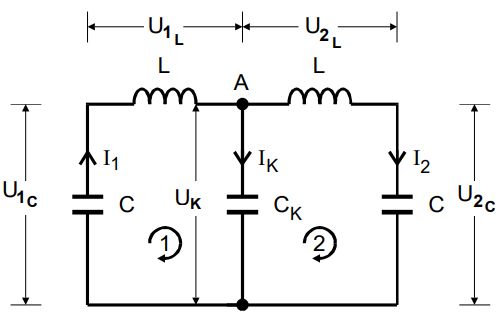
\includegraphics[width = 0.6\textwidth]{content/SkizzegekoppelterSchwingkreis.PNG}
    \caption{In dieser Abbildung ist die Skizze eines kapazitiv gekoppelten Schwingkreises zu sehen. \cite{v355}}
    \label{fig:T_skgS}
\end{figure}
